\section{Antal}
\setbeamertemplate{caption}{\raggedright\insertcaption\par}
\begin{frame}{Introduction}{Antal János Monori\newline<amonor14@student.aau.dk>}
	\begin{figure}[h!]
		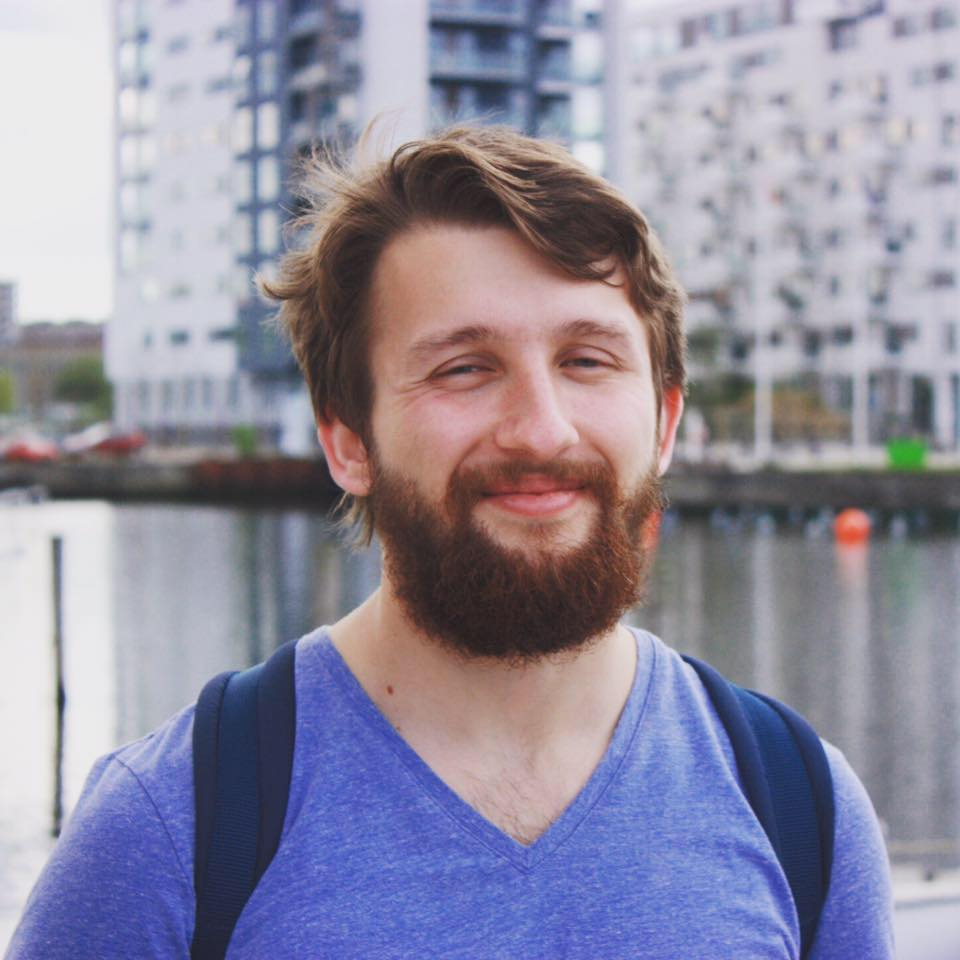
\includegraphics[width=0.3\textwidth]{images/anthony.jpg}
		\caption{Antal János Monori}
		\centering    		
	\end{figure}
\end{frame}

\setbeamertemplate{caption}[default]

\begin{frame}{Overview}{Antal János Monori\newline<amonor14@student.aau.dk>}
	Presentation Agenda
	\begin{itemize}
		\item Introduction
		\item Testing and Prototyping
		\item Future steps
		\item Process analysis
	\end{itemize}
\end{frame}


\begin{frame}{Introduction}{Antal János Monori\newline<amonor14@student.aau.dk>}
	\begin{itemize}
		\item <2-> Mapping and Navigation of unknown terrain
		% Let's decode the title a bit and look at the individual parts a bit more in depth
		\begin{itemize}
			\item <3-> Mapping % idea behind, motivation, problem to solve
			\item <4-> Navigation % idea behind, motivation, problem to solve
			\item <5-> Unknown terrain % idea behind, motivation, problem to solve
		\end{itemize}
		\item <6-> 3D mapping, full autonomous navigation, etc. % what we have in plans for the future development of the idea (short-motivation)
	\end{itemize}
\end{frame}

\begin{frame}{Approach}{Antal János Monori\newline<amonor14@student.aau.dk>}

\end{frame}

\begin{frame}{Components}{Antal János Monori\newline<amonor14@student.aau.dk>}
	
\end{frame}

\begin{frame}{Components - Navigation module}{Antal János Monori\newline<amonor14@student.aau.dk>}
	
\end{frame}

\begin{frame}{Components - Mapping module}{Antal János Monori\newline<amonor14@student.aau.dk>}
	
\end{frame}